\chapter{SHG Yield}
\minitoc

\section{Three layer model for SHG radiation}

In this section we derive the formulas required for the calculation of the SHG
yield, defined by
\begin{equation}\label{uno}
\calr(\omega)=\frac{I(2\omega)}{I^2(\omega)}
,
\end{equation}
with the intensity in the MKS system is given by\cite{boyd}
\begin{equation}\label{dos}
I(\omega)=2n(\go)\epsilon_0c
|E(\omega)|^2
,
\end{equation}
where $n(\omega)=\sqrt{\ge(\go)}$ is the index of refraction with
$\ge(\go)$ the dielectric function, $\ge_0$ is the vacuum permittivity,
and $c$ the speed of light in vacuum.

There are several ways to calculate $R$, one of which is the procedure followed
by Cini \cite{ciniPRB91}. This approach calculates the nonlinear susceptibility
and at the same time the radiated fields. However, we present an alternative
derivation based in the work of Mizrahi and Sipe \cite{mizrahiJOSA88}, since
the derivation of the three-layer-model is straightforward. 
In this scheme, 
we represent the surface by three regions or layers. The first layer
is the vacuum region (denoted by $v$) with a dielectric function $\ge_v(\go)=1$ from
where the fundamental electric field $\bfE_v(\go)$ impinges on the material. 
The second  layer is a thin layer (denoted by $\ell$) of thickness $d$ characterized
by a dielectric function $\ge_\ell(\go)$. Is in this layer where the
second harmonic generation takes place. The third layer is the bulk
region denoted by $b$ and characterized by $\ge_b(\go)$. 
Both the vacuum layer and the
bulk layer are semiinfinite  (see Fig. \ref{3layer}). 

To model the electromagnetic response of the three-layer model 
we follow Ref. \cite{mizrahiJOSA88},
and assume a polarization sheet of the form
\begin{align}\label{m31}
\bfP(\bfr,t)=\boldsymbol{\mathcal{P}}
e^{i\boldsymbol{\kappa}\cdot\bfR}e^{-i\go t}\gd(z-z_\beta)+\mathrm{c.c.}
,
\end{align}
where $\bfR=(x,y)$, $\boldsymbol{\kappa}$ 
is the component of the wave
vector $\boldsymbol{\nu}^{\strut}_\beta$ paralel to the surface, and
$z_\beta$ is the position of the sheet within
medium $\beta$ (see Fig.~\ref{3layer}).
In Ref. \cite{sipeJOSAB87} it has been shown 
that the solution of the Maxwell equations for the radiated fields 
$E_{\beta,p\pm}$ and $E_{\beta,s}$
with $\bfP(\bfr,t)$as a source can be written, at points
$z\neq 0$, as 
\begin{equation}\label{r2}
(E_{\beta,p\pm},E_{\beta,s}) = 
(\frac{\gamma i\tilde\omega^2}{\tilde w_\beta}
\,\hat{\mathbf{p}}_{\beta\pm}\cdot\boldsymbol{\mathcal{P}},
\frac{\gamma i\tilde\omega^2}{\tilde w_\beta}
\,\hat{\mathbf{s}}\cdot\boldsymbol{\mathcal{P}}),
\end{equation} 
where $\gamma=2\pi$ in cgs units and $\gamma=1/2\ge_0$ in MKS units.
Also,
$\hat{\mathbf{s}}$ and $\hat{\mathbf{p}}_{\beta\pm}$ are the unitary vectors for
the $s$ and $p$ polarization of the radiated field, 
respectively, and the $\pm$ refers to upward ($+$) or
downward ($-$) direction of propagation within medium $\beta$, as shown in
Fig.~\ref{3layer}, and $\tilde\go=\go/c$.
Also, $\tilde w_\beta(\omega)=\tilde\go w_\beta$, where
\begin{equation}\label{r3}
w^{\strut}_\beta(\omega)=(\epsilon^{\strut}_\beta(\omega) - \sin^2\theta_0\big)^{1/2},
\end{equation}
where $\theta_0$ is the angle of incidence of $\bfE_v(\go)$, 
and
\begin{equation}\label{r4}
\hat{\mathbf{p}}^{\strut}_{\beta\pm}(\go) =
\frac{\kappa(\go)\hat{\mathbf{z}}\mp \tilde 
  w_\beta(\omega)\hat{\boldsymbol{\kappa}}} 
{\tilde\go n_\beta(\omega)}
=
\frac{\sin\theta_0\hat{\mathbf{z}}\mp 
  w_\beta(\omega)\hat{\boldsymbol{\kappa}}} 
{n_\beta(\omega)}
,
\end{equation}
where $\kappa(\go)=|\boldsymbol{\kappa}|=\tilde\go\sin\theta_0$,
$n_\beta(\go)=\sqrt{\ge_\beta(\go)}$ is
the index of refraction of medium $\beta$, and
$z$ is the direction perpendicular to the surface that 
points towards the vacuum.
We chose the plane of incidence along the  
$\boldsymbol{\kappa}z$ plane, then 
\begin{equation}\label{mc1}
\hat{\boldsymbol{\kappa}}
= \cos\phi\hat{\mathbf{x}} + \sin\phi\hat{\mathbf{y}},
\end{equation}
and
\begin{equation}\label{mmc2}
\hat{\mathbf{s}} = -\sin\phi\hat{\mathbf{x}} + \cos\phi\hat{\mathbf{y}},
\end{equation}
where
$\phi$ the angle with respect to the $x$ axis.

In the three-layer model the nonlinear polarization responsible for 
the second harmonic generation (SHG) is immersed in the thin $\beta=\ell$
layer, and is given by 
\begin{equation}\label{tres}
\mathcal{P}_i(2\omega)=
\left\{
\begin{array}{cc}
\chi_{ijk}(2\go)E_{j}(\omega)E_{k}(\omega) & \text{(cgs units)} \\
\ge_0\chi_{ijk}(2\go)E_{j}(\omega)E_{k}(\omega) & \text{(MKS units)}
\end{array}
\right.
,
\end{equation}
where the  
tensor $\boldsymbol{\chi}(2\go)$ is the surface nonlinear  
dipolar susceptibility and the Cartesian indices $i,j,k$ are summed if repeated. 
Also, $\chi_{ijk}(2\go)=\chi_{ikj}(2\go)$ 
is the intrinsic permutation symmetry
due to the fact that SHG is degenerate in $E_j(\go)$ and $E_k(\go)$.
As it was done in Ref. \cite{mizrahiJOSA88},
in presenting the results Eq.~\eqref{r2}-\eqref{mmc2}
we have taken the
polarization sheet (Eq.~\eqref{m31}) to be oscillating at some frequency
$\go$. However,
 in the following we find it convenient to use $\go$
exclusively to denote the fundamental frequency and
$\boldsymbol{\kappa}$
 to denote the
component of the incident wave vector parallel to the surface. Then
the nonlinear 
generated polarization is oscillating at $\Omega= 2\omega$
and will be characterized
by a wave vector parallel to the surface 
$\bfK=2\boldsymbol{\kappa}$. 
We can carry over
Eqs. \eqref{m31}-\eqref{mmc2} 
simply by replacing the lowercase symbols 
($\go,\tilde\go,\boldsymbol{\kappa},n_\beta,\tilde w_\beta,w_\beta,\hat\bfp_{\beta\pm},\hat\bfs$)  
with uppercase symbols 
($\Omega,\tilde\Omega,\bfK,N_\beta,\tilde W_\beta,W_\beta,\hat\bfP_{\beta\pm},\hat\bfS$),
all evaluated at $2\go$ and
we always have $\hat\bfS=\hat\bfs$.

\begin{figure}[t]
\centering 
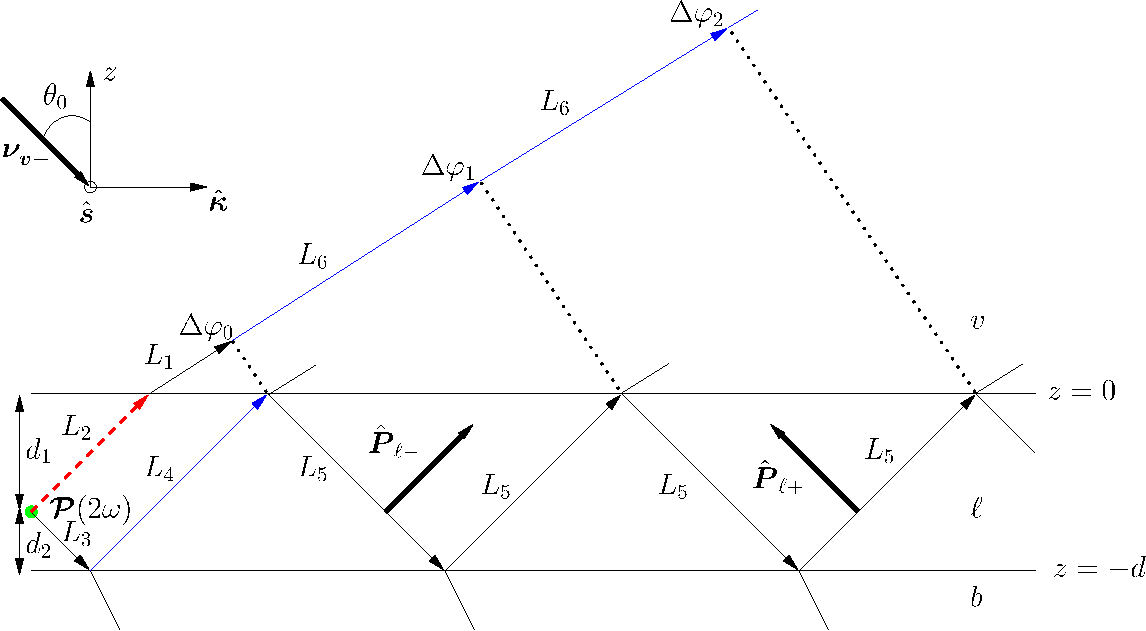
\includegraphics[scale=.5]{figures/multi}
\caption{Sketch of the three layer model for SHG. Vacuum ($v$) is on top with
$\epsilon_v=1$; the layer $\ell$, of thickness $d=d_1+d_2$, is characterized
with $\epsilon_{\ell}(\omega)$, and it is where the SH polarization sheet
$\boldsymbol{\mathcal{P}}(2\omega)$ is located at $z_\ell=d_1$; The bulk $b$ is
described with $\epsilon_{b}(\omega)$. The arrows point along the direction of
propagation, and the $p$-polarization unit vector, $\hat\bfP_{\ell -(+)}$, along
the downward (upward) direction is denoted with a thick arrow. The
$s$-polarization unit vector $\hat\bfs$, points out of the page. The fundamental
field $\bfE(\go)$ is incident from the vacuum side along the
$z\hat{\boldsymbol{\kappa}}$-plane, with $\theta_0$ its angle of incidence and
$\boldsymbol{\nu}_{v-}$ its wave vector. $\Delta\varphi_{i}$ denote the phase
difference of the multiply reflected beams with respect to the first vacuum
transmitted beam (dashed-red arrow), where the dotted lines are perpendicular to
this beam (see the text for details).\label{3layer}}
\end{figure}

To describe the propagation of the SH field, we  see from
Fig. \ref{3layer}, that it is refracted at the 
layer-vacuum interface ($\ell v$), and multiply reflected from the
layer-bulk ($\ell b$)
and layer-vacuum ($\ell v$)
interfaces, thus we can define,
\begin{equation}\label{r5}
\mathbf{T}^{\ell v}
= \hat{\mathbf{s}}T_s^{\ell v}\hat{\mathbf{s}} 
+ \hat{\mathbf{P}}_{v+}T_{p}^{\ell v} \hat{\mathbf{P}}_{\ell +},
\end{equation}
as the tensor for transmission from $\ell v$ interface,
\begin{equation}\label{r6}
\mathbf{R}^{\ell b}
= \hat{\mathbf{s}}R_s^{\ell b}\hat{\mathbf{s}}
+ \hat{\mathbf{P}}_{\ell +}R_{p}^{\ell b} \hat{\mathbf{P}}_{\ell -},
\end{equation} 
as the tensor of reflection from the $\ell b$ interface, 
and
\begin{equation}\label{r6b}
\mathbf{R}^{\ell v}
= \hat{\mathbf{s}}R_s^{\ell v}\hat{\mathbf{s}}
+ \hat{\mathbf{P}}_{\ell -}R_{p}^{\ell v} \hat{\mathbf{P}}_{\ell +},
\end{equation} 
as that of the $\ell v$ interface. 
The Fresnel factors in uppercase letters, $T^{ij}_{s,p}$ and $R^{ij}_{s,p}$,
are evaluated at $2\go$  from the following well known formulas 
\begin{equation}\label{e.f1}
\begin{split}
t_s^{ij}(\omega) &=
\frac{2k_{i}(\omega)}{k_{i}(\omega)+k_{j}(\omega)},
\quad\quad  
t_{p}^{ij}(\omega) =
\frac{2k_{i}(\omega)\sqrt{\epsilon_{i}(\omega)\epsilon_j(\omega)}}
     {k_{i}(\omega)\epsilon_{j}(\omega)+k_{j}(\omega)\epsilon_{i}(\omega)},\\
r_s^{ij}(\omega) &=
\frac{k_{i}(\omega) - k_{j}(\omega)}
     {k_{i}(\omega) + k_{j}(\omega)},
\quad\quad 
r_{p}^{ij}(\omega) =
\frac{k_{i}(\omega)\epsilon_{j}(\omega) - k_{j}\epsilon_{i}(\omega)}
     {k_{i}(\omega)\epsilon_{j}(\omega) + k_{j}(\omega)\epsilon_{i}(\omega)}. 
\end{split}
\end{equation}
From these expressions one can show that,
\begin{align}\label{mf}
1 + r^{\ell b}_{s} &= t^{\ell b}_{s}\nonumber\\
1 + r^{\ell b}_{p}
&= \frac{n_b}{n_\ell}
t^{\ell b}_{p} 
\nonumber\\
1 - r^{\ell b}_{p}
&= \frac{n_\ell}{n_b}
   \frac{w_{b}}{w_{\ell}}t^{\ell b}_{p}\\
t^{\ell v}_{p} &= \frac{w_{\ell}}{w_{v}}t^{v\ell}_{p}\nonumber\\
t^{\ell v}_{s} &= \frac{w_{\ell}}{w_{v}}t^{v\ell}_{s}\nonumber 
.
\end{align}


\subsection{Multiple SH reflections}

The SH field $\bfE(2\go)$ radiated by the SH polarization 
$\boldsymbol{\mathcal{P}}(2\go)$
will radiate directly into vacuum and also into the bulk,
where it will be reflected back at the thin-layer-bulk interface into 
the thin layer again and this beam will be multiple-transmitted and 
reflected as shown in Fig.~\ref{3layer}. 
As the two beams propagate a phase difference will develop between
them, according to
\begin{align}\label{m99}
\gD\varphi_m&=\tilde\gO\Big((L_3+L_4+2mL_5)N_\ell
-\big( L_2N_\ell+(L_1+mL_6)N_v\big)
\Big)
\nonumber\\
&=\gd_0 + m\gd\quad m=0,1,2,\ldots
,
\end{align}
where
\begin{align}\label{m97}
\gd_0=8\pi\left(\frac{d_2}{\lambda_0}\right)\sqrt{n^2_\ell(2\go)-\sin^2\theta_0}
,
\end{align}
\begin{align}\label{m96}
\gd=8\pi\left(\frac{d}{\lambda_0}\right)\sqrt{n^2_\ell(2\go)-\sin^2\theta_0}
,
\end{align}
where $\lambda_0$ is the wavelength of the fundamental field in
vacuum, $d$ the thickness of layer $\ell$ and $d_2$ the distance of
$\boldsymbol{\mathcal{P}}(2\omega)$  
from the $\ell b$ interface 
(see Fig.~\ref{3layer}).
We see that
$\gd_0$ is the phase difference of 
the first and second transmitted beams, and $m\gd$ that of the first 
and  third ($m=1$), fourth ($m=2$), etc. beams (see 
Fig.~\ref{3layer}). 

To take into account the multiple reflections of the generated SH
field in the layer $\ell$, we proceed as follows. We show the algebra
for the $p$-polarized SH field, the $s$-polarized field could be
worked out along the same steps. The multiple-reflected $\bfE_p(2\go)$
field is given by
\begin{equation}\label{m7}
\begin{split}
\mathbf{E}(2\omega) 
&=  
E_{p+}(2\omega)\mathbf{T}^{\ell v}\cdot\hat{\mathbf{P}}_{\ell +}
+ E_{p-}(2\omega)\mathbf{T}^{\ell v}
\cdot\mathbf{R}^{\ell b}\cdot\hat{\mathbf{P}}_{\ell-}e^{i\gD\varphi_0}
+ E_{p-}(2\omega)\mathbf{T}^{\ell v}
\cdot\mathbf{R}^{\ell b}\cdot\mathbf{R}^{\ell v}
\cdot\mathbf{R}^{\ell b}\cdot\hat{\mathbf{P}}_{\ell-}e^{i\gD\varphi_1}
\\
&
+ E_{p-}(2\omega)\mathbf{T}^{\ell v}
\cdot\mathbf{R}^{\ell b}\cdot\mathbf{R}^{\ell v}
\cdot\mathbf{R}^{\ell b}\cdot\mathbf{R}^{\ell v}
\cdot\mathbf{R}^{\ell b}\cdot\hat{\mathbf{P}}_{\ell-}e^{i\gD\varphi_2}
+\cdots 
\\
&= 
E_{p+}(2\omega)\mathbf{T}^{\ell v}\cdot\hat{\mathbf{P}}_{\ell +}
+ E_{p-}(2\omega) \mathbf{T}^{\ell v}
\cdot\sum_{m=0}^\infty  
\big(
\mathbf{R}^{\ell b}\cdot\mathbf{R}^{\ell v} 
e^{i\gd}\Big)^m 
\cdot\mathbf{R}^{\ell b}\cdot\hat{\mathbf{P}}_{\ell-}e^{i\gd_0}
.
\end{split}
\end{equation} 
From Eqs.~\eqref{r5}-\eqref{r6b} is easy to show
that
\begin{align}\label{m1}
\mathbf{T}^{\ell v}\cdot 
\Big(\mathbf{R}^{\ell b}\cdot\mathbf{R}^{\ell v}\Big)^n 
\cdot \mathbf{R}^{\ell b}
&=
\hat{\mathbf{s}}
T^{\ell v}_s\Big(R^{\ell b}_sR^{\ell v}_s\Big)^n 
 R^{\ell b}_s 
\hat{\mathbf{s}}
+
\hat{\mathbf{P}}_{v+}
T^{\ell v}_p\Big(R^{\ell b}_pR^{\ell v}_p\Big)^n 
 R^{\ell b}_p 
\hat{\mathbf{P}}_{\ell-}
,
\end{align}
then,
\begin{equation}\label{m7}
\begin{split}
\mathbf{E}(2\omega) 
&= 
\hat{\mathbf{P}}_{\ell +}T^{\ell v}_p
\Big(
E_{p+}(2\omega) 
+
\frac{R^{\ell b}_pe^{i\gd_0}}{1+R^{v\ell}_pR^{\ell b}_pe^{i\gd}}
E_{p-}(2\omega) 
\Big)
,
\end{split}
\end{equation}
where we used $R^{ij}_{s,p}=-R^{ji}_{s,p}$.
Using Eq.~\eqref{r2}, we can readily write
\begin{equation}\label{mr8}
\mathbf{E}(2\omega) = \frac{\gamma i\tilde{\Omega}}{W_{\ell}}
\mathbf{H}_{\ell}\cdot\boldsymbol{\mathcal{P}}(2\omega),
\end{equation}
where
\begin{equation}\label{mr9}
\mathbf{H}_{\ell}
= \hat{\mathbf{s}}\,T_s^{\ell v}
\left(1+
R^M_s
\right)
\hat{\mathbf{s}}
+ \hat{\mathbf{P}}_{v+}T_{p}^{\ell v}
\left(
\hat{\mathbf{P}}_{\ell +} +
R^M_p
 \hat{\mathbf{P}}_{\ell -}
\right). 
\end{equation}
and
\begin{align}\label{m61}
R^M_l\equiv\frac{R^{\ell b}_le^{i\gd_0}}{1+R^{v\ell}_l R^{\ell b}_l e^{i\gd}}
\quad l=s,p
,
\end{align}
is defined as the multiple  ($M$) reflection coefficient.
To make touch with the work of Ref. \cite{mizrahiJOSA88} where
$\boldsymbol{\mathcal{P}}(2\omega)$ is located on top of the
vacuum-surface interface and only the vacuum radiated beam and the
first (and only) reflected beam need to be considered, we take
$\ell=v$ and $d_2=0$, then 
$T^{\ell v}=1$, $R^{v\ell}=0$ and $\gd_0=0$, with which
$R^M_l=R^{vb}_l$. 
Thus, Eq.~\eqref{mr9} coincides with Eq. (3.8) of
Ref. \cite{mizrahiJOSA88}. 

\subsection{Multiple reflections for the linear field}
\begin{figure}[t]
\centering 
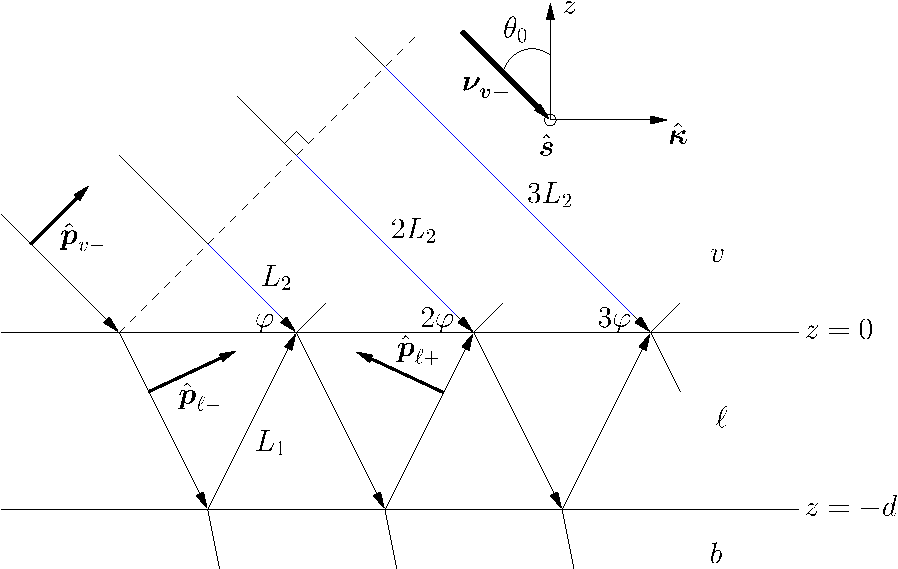
\includegraphics[scale=.5]{figures/linear-field}
\caption{(color on line) Sketch for the multiple reflected  fundamental field
$\bfE(\go)$, which impinges from the vacuum side along the
$z\hat{\boldsymbol{\kappa}}$-plane, with $\theta_0$ and $\boldsymbol{\nu}_{v-}$
its angle of incidence and wave vector, respectively. The arrows point along the
direction of propagation. The $p$-polarization unit vectors, $\hat\bfp_{\beta
\pm}$, along the downward (-) or upward (+) direction are denoted with thick
arrows, where $\beta=v$ or $\ell$. The $s$-polarization unit vector $\hat\bfs$
points out of the page, and $(1,2,3,\dots)\phi$ denotes the phase difference for
the multiply reflected beams with respect to the incident field, where the
dotted line is perpendicular to this beam (see the text for
details).\label{linear}}
\end{figure}

Similar to the SH field, here we consider the multiple reflections of
the fundamental field $\bfE(\go)$ inside the thin $\ell$ layer.
In Fig.~\ref{linear} we show the situation where $\bfE(\go)$
impinges from the vacuum side with an angle of incidence $\theta_0$. 
As the first transmitted beam is multiply reflected from the $\ell b$ and the
$\ell v$ interfaces, it accumulates a phase difference of $n\phi$,
with $n=1,2,3,\ldots$, given by
\begin{align}\label{mphi}
\phi&=\frac{\go}{c}(2L_1n_\ell-L_2n_v)
\nonumber\\
&=4\pi\left(\frac{d}{\lambda_0}\right)\sqrt{n^2_\ell-\sin^2\theta_0}
,
\end{align}
where $n_v=1$. Besides the equivalent of Eqs.~\eqref{r6} and
\eqref{r6b}, for $\go$, we also need
\begin{align}\label{mvv}
\mathbf{t}^{v\ell}
= \hat{\mathbf{s}}t_s^{v\ell}\hat{\mathbf{s}} 
+ \hat{\mathbf{p}}_{\ell -}t_{p}^{v\ell} \hat{\mathbf{p}}_{v -}
,
\end{align}
to write
\begin{align}\label{mcvew}
\bfE(\go)
&=E_0\Big[
\bft^{v\ell}
+
\bfr^{\ell b}\cdot\bft^{v\ell}e^{i\phi}
+
\bfr^{\ell b}\cdot\bfr^{\ell v}\cdot \bfr^{\ell b}\cdot\bft^{v\ell} e^{i2\phi}
+
\bfr^{\ell b}\cdot\bfr^{\ell v}\cdot 
\bfr^{\ell b}\cdot\bfr^{\ell v}
\cdot \bfr^{\ell b}\cdot\bft^{v\ell} e^{i3\phi}
+\cdots\Big]\cdot\bfe^{\mathrm{in}}
\nonumber\\
&=E_0\Big[
1
+
\Big(1+
\bfr^{\ell b}\cdot\bfr^{\ell v}e^{i\phi}
+
(\bfr^{\ell b}\cdot\bfr^{\ell v})^2e^{i2\phi}+\cdots
\Big)\cdot
\bfr^{\ell b}e^{i\phi}
\Big]\cdot \bft^{v\ell}\cdot\bfe^{\mathrm{in}}
\nonumber\\
&=
E_0\Big[\hat\bfs t^{v\ell}_s(1+r^M_s)\hat\bfs
+
t^{v\ell}_p\left(\hat\bfp_{\ell-}+\hat\bfp_{\ell+}r^{M}_p
\right)\hat\bfp_{v-}
\Big]\cdot\bfe^{\mathrm{in}}
\end{align}
where
\begin{align}\label{mvrm}
r^M_l=\frac{r^{\ell b}_le^{i\phi}}{1+r^{v\ell}_lr^{\ell
  b}_le^{i\phi}}\quad l=s,p
.
\end{align}
We define $\bfE^l(\go)\equiv E_0\bfe^{\go,l}_\ell$ ($l=s,p$),
where using Eq.~\eqref{r4}, we obtain that
\begin{eqnarray}\label{mcvep}
\bfe^{\go,p}_\ell=\frac{t^{v\ell}_p}{n_\ell}\left( 
r^{M+}_p\sin\theta_0\hat\bfz  
+ 
r^{M-}_pw_\ell\hat{\boldsymbol{\kappa}}
\right)  
,
\end{eqnarray} 
for $p$-input polarization, i.e. $\bfe^{\mathrm{in}}=\hat\bfp_{v-}$, 
and
\begin{eqnarray}\label{mcvep}
\bfe^{\go,s}_\ell=t^{v\ell}_sr^{M+}_s\hat\bfs
,
\end{eqnarray}
for $s$-input polarization, i.e. $\bfe^{\mathrm{in}}=\hat\bfs$,
where
\begin{eqnarray}\label{mvc}
r^{M\pm}_l=1\pm r^M \quad l=s,p.
\end{eqnarray}
\subsection{SHG Yield}

The magnitude of the radiated field is given by
$E(2\omega)=\hat{\mathbf{e}}^{\mathrm{out}}\cdot\mathbf{E}(2\omega)$, where
$\hat{\mathbf{e}}^{\mathrm{out}}$ is the polarization vector of the radiated
field, for instance $\hat{\mathbf{s}}$ or $\hat{\mathbf{P}}_{v+}$. Then, we
write
\begin{equation}\label{m1}
\begin{split}
\hat{\mathbf{P}}_{\ell +} + R^M_p\hat{\mathbf{P}}_{\ell -}
&= \frac{\sin\theta_0\hat{\mathbf{z}} - W_{\ell}\hat{\boldsymbol{\kappa}}}
        {N_{\ell}}
 + R^M_p
   \frac{\sin\theta_0\hat{\mathbf{z}} + W_{\ell}\hat{\boldsymbol{\kappa}}}
        {N_{\ell}}
\\
&= \frac{1}{N_{\ell}}
\left(
\sin\theta_0R^M_{p+}\hat{\mathbf{z}}
- K_{\ell}R^M_{p-}\hat{\boldsymbol{\kappa}}
\right)
,
\end{split}
\end{equation}
where
\begin{align}\label{rm}
R^{M\pm}_l\equiv 1 \pm R^M_l \quad l=s,p
.
\end{align}
 Using Eq.~\eqref{mf}
 we write Eq.~\eqref{mr8} as
\begin{equation}\label{r10}
E(2\omega) = \frac{2\gamma i \omega}{cW_\ell}
\hat{\mathbf{e}}^{\mathrm{out}}\cdot 
\mathbf{H}_{\ell}\cdot 
\boldsymbol{\mathcal{P}}(2\omega) 
= \frac{2\gamma i \omega}{cW_v}
 \mathbf{e}^{\,2\omega}_{\ell}\cdot\boldsymbol{\mathcal{P}}(2\omega). 
\end{equation}
\begin{equation}\label{r12mm}
\begin{split}
\mathbf{e}^{2\omega}_{\ell} &=\hat{\mathbf{e}}^{\mathrm{out}}\cdot 
\Bigg[
\hat{\mathbf{s}}T_{s}^{v\ell}R^{M+}_s\hat{\mathbf{s}} + 
\hat{\mathbf{P}}_{v+}
\frac{T^{v\ell}_{p}}
     {N_\ell}
\left(
\sin\theta_0R^{M+}_p\hat{\mathbf{z}}
- W_{\ell}R^{M-}_p\hat{\boldsymbol{\kappa}}
\right) 
\Bigg]
. 
\end{split}
\end{equation}  
 We pause here to reduce above result to the case where the nonlinear
polarization $\mathbf{P}(2\omega)$ radiates from vacuum instead from the layer
$\ell$. For such case we simply take $\epsilon_{\ell}(2\omega)=1$ and $\ell=v$
($T^{\ell v}_{s,p}=1$), to get
\begin{equation}\label{r13}
\mathbf{e}^{\,2\omega}_{v} = \hat{\mathbf{e}}^{\mathrm{out}}
\cdot\left[
\hat{\mathbf{s}}T_s^{v b}\hat{\mathbf{s}} + \hat{\mathbf{P}}_{v+}
\frac{T^{v b}_{p}}{\sqrt{\epsilon_{b}(2\omega)}}
\left(
  \epsilon_{b}(2\omega)\sin\theta_0\hat{\mathbf{z}}
  - W_{b}\hat{\boldsymbol{\kappa}}
\right) 
\right] 
,
\end{equation}
which agrees with Eq. (3.10) of Ref. \cite{mizrahiJOSA88}.

In the three layer model the SH polarization $\calbp(2\go)$ is located in layer $\ell$,
where we evaluate the fundamental field required in Eq. \eqref{tres}.
We write
\begin{equation}\label{m2}
\mathbf{E}_{\ell}(\omega)=E_0\left(
\hat{\mathbf{s}} t^{v\ell}_s(1+r^{\ell b}_s)\hat{\mathbf{s}}
+
\hat{\mathbf{p}}_{\ell-}
 t^{v\ell}_{p}
\hat{\mathbf{p}}_{v-}
+
\hat{\mathbf{p}}_{\ell+}
t^{v\ell}_{p}r^{\ell b}_{p}
\hat{\mathbf{p}}_{v-}
\right)\cdot\hat{\mathbf{e}}^{\mathrm{in}}=E_0\mathbf{e}^\omega_{\ell}
,
\end{equation} 
where $\bfe^{\mathrm{in}}$ is the $s$ ($\hat\bfs$) or $p$
($\hat\bfp_{v-}$)
incoming polarization of
the fundamental electric field. 
Above field is composed of the transmitted field and its first
reflection from the $\ell b$ interface for $s$ and $p$ polarizations.
The fundamental field, once inside the layer $\ell$ will be multiply
reflected at the $\ell v$ and $\ell b$ interfaces, however each
reflection will diminish the intensity of the fundamental field, and as the SHG
yield goes with the square of this field, the contribution of the
subsequent reflections, other than the one considered in
Eq.~\eqref{m2},  could be safely neglected.
From Eq.~\eqref{mf}
we find that
\begin{equation}\label{m12}
\mathbf{e}^{\omega}_{\ell}
= \left[
\hat{\mathbf{s}}t_{s}^{v\ell}t_{s}^{\ell b}\hat{\mathbf{s}} 
+ \frac{t^{v\ell}_{p}t^{\ell b}_{p}}
       {n^2_\ell n_b}
\left(
  n^2_b
\sin\theta_0\hat{\mathbf{z}}
+ n^2_\ell w_b\hat{\boldsymbol{\kappa}}
\right)
\hat{\mathbf{p}}_{v-}
\right]
\cdot\hat{\mathbf{e}}^{\mathrm{in}}.  
\end{equation}  
Again, to touch base with Ref. \cite{mizrahiJOSA88},
if we would like to evaluate the fields in the bulk, instead of the layer
$\ell$, we simply take 
$n_\ell=n_b,\,(t^{\ell b}_{s,p}=1$), to obtain
\begin{equation}\label{m13}
\mathbf{e}^{\omega}_{b}
= \left[
\hat{\mathbf{s}}t_{s}^{vb}\hat{\mathbf{s}}
+ \frac{t^{vb}_{p}}{n_b}
\left(
\sin\theta_0\hat{\mathbf{z}} + w_b\hat{\boldsymbol{\kappa}}
\right) 
\hat{\mathbf{p}}_{v-}
\right]
\cdot\hat{\mathbf{e}}^{\mathrm{in}},  
\end{equation} 
that is in agreement with Eq. (3.5) of Ref. \cite{mizrahiJOSA88}.
Then,
 we can write Eq. \eqref{tres} as
\begin{equation}\label{m4}
\boldsymbol{\mathcal{P}}(2\omega) = 
\left\{
\begin{array}{cc}  
E^{2}_{0}\,\boldsymbol{\chi}:\mathbf{e}^{\omega}_{\ell}\mathbf{e}^{\omega}_{\ell}
& \text{(cgs units)} \\
\ge_0E^{2}_{0}\,\boldsymbol{\chi}:\mathbf{e}^{\omega}_{\ell}\mathbf{e}^{\omega}_{\ell}
& \text{(MKS units)} \\
\end{array}
\right.
,
\end{equation}
where $E_0$ is the intensity of the fundamental electric field.
Finally, with above equation we write Eq.~\eqref{r10} as
\begin{equation}\label{mr10}
E(2\omega) 
= \frac{2\eta i \omega}{cW_v}
\mathbf{e}^{2\omega}_{\ell}\cdot\boldsymbol{\chi}:\mathbf{e}^{\omega}_{\ell}
\mathbf{e}^{\omega}_{\ell}
,
\end{equation}
where $\eta=2\pi$ for cgs units and $\eta=1/2$ for MKS units.
To ease on the notation, we define
\begin{align}\label{mc0}
\Upsilon_{\mathrm{iO}}
\equiv 
\mathbf{e}^{2\omega}_{\ell}\cdot\boldsymbol{\chi}:\mathbf{e}^{\omega}_{\ell}
\mathbf{e}^{\omega}_{\ell}
,
\end{align}
where i stands for the incoming polarization of the fundamental
electric field given by $\hat\bfe^{\mathrm{in}}$ in Eq.~\eqref{m12},
and O for the outgoing polarization of the SH electric field
given by $\hat\bfe^{\mathrm{out}}$ in Eq.~\eqref{r12mm}.

From Eqs. \eqref{uno} and \eqref{dos} we obtain that
in the cgs units ($\eta=2\pi$)
\begin{align}\label{r01}
|E(2\omega)|^2 
&= |E_{0}|^4\frac{16\pi^{2}\omega^{2}}{c^{2}W^2_v}
\left\vert  
\Upsilon_{\mathrm{iO}}
\right\vert^{2}
\nonumber\\
\frac{c}{2\pi}|\sqrt{N_v}E(2\omega)|^{2} 
&=
\frac{32\pi^{3}\omega^{2}}{c^{3}\cos^2\theta_0}
\left\vert  
\frac{\sqrt{N_v}}{n^2_\ell}
\Upsilon_{\mathrm{iO}}
\right\vert^{2} 
\left(\frac{c}{2\pi}|\sqrt{n_\ell}E_{0}|^{2}\right)^{2},
\nonumber\\ 
I(2\omega) 
&= \frac{32\pi^{3}\omega^{2}}{c^{3}\cos^2\theta_0}
\left\vert  
\frac{\sqrt{N_v}}{n^2_\ell}
\Upsilon_{\mathrm{iO}}
\right\vert^{2}I^{2}(\omega),
\nonumber\\
\calr_{\mathrm{iO}}(2\omega) 
&= 
\frac{32\pi^{3}\omega^{2}}{c^{3}\cos^2\theta_0}
\left\vert  
\frac{1}{n_\ell}
\Upsilon_{\mathrm{iO}}
\right\vert^{2}
,
\end{align} 
and in MKS units ($\eta=1/2$)
\begin{align}\label{r01m}
|E(2\omega)|^2 
&= |E_{0}|^4
\frac{\omega^{2}}{c^{2}W^2_v}
\left\vert  
\Upsilon_{\mathrm{iO}}
\right\vert^{2}
\nonumber\\
2\ge_0c|\sqrt{N_v}E(2\omega)|^{2} 
&=
\frac{2\ge_0\omega^{2}}{c\cos^2\theta_0}
\left\vert  
\frac{\sqrt{N_v}}{n^2_\ell}
\Upsilon_{\mathrm{iO}}
\right\vert^{2} 
\frac{1}{4\ge^2_0c^2}\left(2\ge_0c|\sqrt{n_\ell}E_{0}|^{2}\right)^{2},
\nonumber\\ 
I(2\omega) 
&= 
\frac{\omega^{2}}{2\ge_0c^3\cos^2\theta_0}
\left\vert  
\frac{\sqrt{N_v}}{n^2_\ell}
\Upsilon_{\mathrm{iO}}
\right\vert^{2}I^{2}(\omega),
\nonumber\\
\calr_{\mathrm{iO}}(2\omega) 
&= \frac{\omega^{2}}{2\ge_0c^3\cos^2\theta_0}
\left\vert  
\frac{1}{n_\ell}
\Upsilon_{\mathrm{iO}}
\right\vert^{2} 
,
\end{align} 
\begin{equation}\label{mc6}
\calr_{\mathrm{iO}}(2\omega) 
\left\{
\begin{array}{cc} 
\frac{32\pi^{3}\omega^{2}}{c^{3}\cos^2\theta_0}
\left\vert  
\frac{1}{n_\ell}
\Upsilon_{\mathrm{iO}}
\right\vert^{2} 
& \text{(cgs units)} \\
\frac{\omega^{2}}{2\ge_0c^3\cos^2\theta_0}
\left\vert  
\frac{1}{n_\ell}
\Upsilon_{\mathrm{iO}}
\right\vert^{2} 
& \text{(MKS units)} 
\end{array}
\right.
,
\end{equation}
as the SHG yield, where $N_v=1$ and $W_v=\cos\theta_0$.
In the MKS unit system $\boldsymbol{\chi}$ is given in m$^2$/V, since
it is a surface second order nonlinear susceptibility, and
$\calr_{\mathrm{iO}}$ is given in m$^2$/W. 


\verb=tal vez esto al apendice=
At this point we mention that to recover the results of Ref.
\cite{mizrahiJOSA88} which are equivalent of those of Ref. \cite{sipePRB87}, we
take $\mathbf{e}^{2\omega}_{\ell}\to \mathbf{e}^{2\omega}_v$,
$\mathbf{e}^{\omega}_{\ell}\to \mathbf{e}^{\omega}_{b}$, 
and then
\begin{equation}\label{m69}
\calr(2\omega) =
\frac{32\pi^{3} \omega^{2}}{c^{3}\cos^{2}\theta_0}
\left\vert
\mathbf{e}^{\,2\omega}_{v}\cdot\boldsymbol{\chi}:
\mathbf{e}^{\omega}_{b}\mathbf{e}^{\omega}_{b}
\right\vert^{2} 
,
\end{equation}
will give the SHG yield of a nonlinear polarization sheet radiating from vacuum
on top of the surface and where the fundamental field is evaluated below the
surface that is characterized by $\epsilon_{b}(\omega)$.


\section{One SH Reflection}
Therefore, the total radiated field at 
$2\omega$ is 
\begin{equation}\label{r7}
\begin{split}
\mathbf{E}(2\omega)  
&= E_s(2\omega)  
\left(
\mathbf{T}^{\ell v} + \mathbf{T}^{\ell v}\cdot\mathbf{R}^{\ell b}
\right)  
\cdot\hat{\mathbf{s}}\nonumber\\
&+ E_{p+}(2\omega)\mathbf{T}^{\ell v}\cdot\hat{\mathbf{P}}_{\ell +}
 + E_{p-}(2\omega)\mathbf{T}^{\ell v}
\cdot\mathbf{R}^{\ell b}\cdot\hat{\mathbf{P}}_{\ell-}.  
\end{split}
\end{equation} 
The first term is  the transmitted $s$-polarized field, the second one is the 
reflected and then transmitted $s$-polarized field and the third and fourth 
terms are the equivalent fields for $p$-polarization. The transmission is from 
the layer into vacuum, and the reflection between the layer and the bulk. After 
some simple algebra, we obtain 
\begin{equation}\label{r8}
\mathbf{E}(2\omega) = \frac{2\pi i\tilde{\Omega}}{K_{\ell}}
\mathbf{H}_{\ell}\cdot\boldsymbol{\mathcal{P}}(2\omega),
\end{equation} 
where,
\begin{equation}\label{r9}
\mathbf{H}_{\ell}
= \hat{\mathbf{s}}\,T_s^{\ell v}\left(1+R_s^{\ell b}\right)\hat{\mathbf{s}}
+ \hat{\mathbf{P}}_{v+}T_{p}^{\ell v}
\left(
\hat{\mathbf{P}}_{\ell +} +R_{p}^{\ell b}\hat{\mathbf{P}}_{\ell -}
\right). 
\end{equation}

%%%%%%%%%%%%%%%%%%%%%%%%%%%%%%%%%%%%%%%%%%%%%%%%%%%%%%%%%%%%%%%%
%%%%%%%%%%%%%%%%%%%%%%%%%%%%%%%%%%%%%%%%%%%%%%%%%%%%%%%%%%%%%%%%
%%%%%%%%%%%%%%%%%%%%%%%%%%%%%%%%%%%%%%%%%%%%%%%%%%%%%%%%%%%%%%%%

\section{\texorpdfstring{$\mathcal{R}$}{R} for different polarization cases}

\subsection{\texorpdfstring{$\mathcal{R}_{pP}$}{RpP}}

We develop five different scenarios for $\mathcal{R}_{pP}$ that explore
different cases for where the polarization and fundamental fields are located.
In all these scenarios, we use
$\hat{\mathbf{e}}^{\mathrm{in}}=\hat{\mathbf{p}}_{v-}$ in Eq. \eqref{m12}, and
$\hat{\mathbf{e}}^{\mathrm{out}}=\hat{\mathbf{P}}_{v+}$ in Eq.
\eqref{r12}.

This scenario involves $\mathcal{P}(2\omega)$ and the fundamental fields to be
taken in a thin layer of material below the surface, which we designate as
$\ell$. Thus,
\begin{equation*}\label{m80}
\mathbf{e}^{\,2\omega}_{\ell}\cdot\boldsymbol{\chi}:
\mathbf{e}^\omega_{\ell}\mathbf{e}^\omega_{\ell}
\equiv\Gamma^{\ell}_{pP}\,r^{\ell}_{pP}
,
\end{equation*}
where
\begin{align}\label{m81}
r^{\ell}_{pP} &=
\epsilon_{b}(2\omega)\sin\theta_{\mathrm{in}}
\Big(
  \epsilon^2_{b}(\omega)\sin^2\theta_{\mathrm{in}}\chi_{zzz}
+ \epsilon^2_{\ell}(\omega)k^2_{b}\chi_{zxx}
\Big)\\
&- \epsilon_{\ell}(2\omega)\epsilon_{\ell}(\omega)k_{b}K_{b}
\Big(
  2\epsilon_{b}(\omega)\sin\theta_{\mathrm{in}}\chi_{xxz}
+ \epsilon_{\ell}(\omega)k_{b}\chi_{xxx}\cos(3\phi) 
\Big),\nonumber
\end{align}
and  
\begin{equation}\label{m79}
\Gamma^{\ell}_{pP}=
\frac{T_{p}^{\ell v}T^{\ell b}_{p}}
     {\epsilon_{\ell}(2\omega)\sqrt{\epsilon_{b}(2\omega)}}
\left(
\frac{t_{p}^{v\ell}t^{\ell b}_{p}}
     {\epsilon_{\ell}(\omega)\sqrt{\epsilon_{b}(\omega)}}
\right)^{2} 
.  
\end{equation}


\subsection{\texorpdfstring{$\mathcal{R}_{pS}$}{RpS}}

To obtain $R_{pS}(2\omega)$ we use
$\hat{\mathbf{e}}^{\mathrm{in}}=\hat{\mathbf{p}}_{v-}$ in Eq. \eqref{m12}, and
$\hat{\mathbf{e}}^{\mathrm{out}}=\hat{\mathbf{S}}$ in Eq. \eqref{r12}. We also
use the unit vectors defined in Eqs. \eqref{eq:kappavec} and
\eqref{eq:svec}. Substituting, we get
\begin{equation*}
\mathbf{e}^{\,2\omega}_{\ell}\cdot
\boldsymbol{\chi}:\mathbf{e}^\omega_{\ell}\mathbf{e}^\omega_{\ell}
\equiv\Gamma^{\ell}_{sP}\, r^{\ell}_{sP},
\end{equation*}
where
\begin{equation}
r^{\ell}_{pS}
= -\epsilon^{2}_{\ell}(\omega)k^{2}_{b}\sin3\phi\chi_{xxx},
\end{equation} 
and  
\begin{equation}
\Gamma^{\ell}_{pS} =
T^{v\ell}_{s}T^{\ell b}_{s}\left(\frac{t^{v\ell}_{p}t^{\ell b}_{p}}
      {\epsilon_{\ell}(\omega)\sqrt{\epsilon_{b}(\omega)}}\right)^{2}.
\end{equation} 
In order to reduce above result to that of Ref. \cite{mizrahiJOSA88} and
\cite{sipePRB87},  we take the $2\omega$ radiations factors for vacuum by
taking $\ell=v$, thus $\epsilon_{\ell}(2\omega)=1$, $T^{v\ell}_{s}=1$,
$T^{\ell b}_{s}=T^{vb}_{s}$, and the fundamental field inside medium $b$ by
taking $\ell=b$, thus $\epsilon_{\ell}(\omega)=\epsilon_{b}(\omega)$,
$t^{v\ell}_{p}=t^{vb}_{p}$, and $t^{\ell b}_{p}=1$. With these choices,
\begin{equation*}
r^{b}_{pS} = -k^{2}_{b}\sin3\phi\chi_{xxx},
\end{equation*} 
and 
\begin{equation*}
\Gamma^{b}_{pS} =
T^{vb}_{s}
\left(
\frac{t^{vb}_{p}}{\sqrt{\epsilon_{b}(\omega)}}
\right)^{2}.  
\end{equation*} 


\subsection{\texorpdfstring{$\mathcal{R}_{sP}$}{RsP}}

To obtain $R_{sP}(2\omega)$ we use
$\hat{\mathbf{e}}^{\mathrm{in}}=\hat{\mathbf{s}}$ in Eq. \eqref{m12}, and
$\hat{\mathbf{e}}^{\mathrm{out}}=\hat{\mathbf{P}}_{v+}$ in Eq. \eqref{r12}. We
also use the unit vectors defined in Eqs. \eqref{eq:kappavec} and
\eqref{eq:svec}. Substituting, we get
\begin{equation*}
\mathbf{e}^{\,2\omega}_{\ell}\cdot
\boldsymbol{\chi}:\mathbf{e}^\omega_{\ell}\mathbf{e}^\omega_{\ell}
\equiv\Gamma^{\ell}_{sP}\, r^{\ell}_{sP},
\end{equation*}
where
\begin{equation}
r^{\ell}_{sP}
= \epsilon_{b}(2\omega)\sin\theta_{\mathrm{in}}\chi_{zxx}
+ \epsilon_{\ell}(2\omega)K_{b}\chi_{xxx}\cos3\phi,
\end{equation} 
and  
\begin{equation}
\Gamma^{\ell}_{sP}=
\frac{T_{p}^{\ell v}T^{\ell b}_{p}\left(t_s^{v\ell}t^{\ell b}_s\right)^2}
     {\epsilon_{\ell}(2\omega)\sqrt{\epsilon_{b}(2\omega)}}.  
\end{equation} 
In order to reduce above result to that of Ref. \cite{mizrahiJOSA88} and
\cite{sipePRB87}, we take the $2\omega$ radiations factors for vacuum by
taking $\ell=v$, thus $\epsilon_{\ell}(2\omega)=1$, $T^{v\ell}_{p}=1$,
$T^{\ell b}_{p}=T^{vb}_{p}$, and the fundamental field inside medium $b$ by
taking $\ell=b$, thus $\epsilon_{\ell}(\omega)=\epsilon_{b}(\omega)$,
$t^{v\ell}_s=t^{vb}_s$, and $t^{\ell b}_s=1$. With these choices,
\begin{equation*}
r^{b}_{sP} = \epsilon_{b}(2\omega)\sin\theta_{\mathrm{in}}\chi_{zxx}
+ K_{b}\chi_{xxx}\cos3\phi,
\end{equation*} 
and 
\begin{equation*}
\Gamma^{b}_{sP} =
\frac{T^{v b}_{p}(t_s^{vb})^{2}}{\sqrt{\epsilon_{b}(2\omega)}}.  
\end{equation*}


\subsection{\texorpdfstring{$\mathcal{R}_{sS}$}{RsS}}

For $\mathcal{R}_{sS}$ we have that
$\hat{\mathbf{e}}^{\mathrm{in}}=\hat{\mathbf{s}}$ and
$\hat{\mathbf{e}}^{\mathrm{out}}=\hat{\mathbf{S}}$. This leads to
\begin{equation*}
\mathbf{e}^{\,2\omega}_{\ell}\cdot
\boldsymbol{\chi}:\mathbf{e}^\omega_{\ell}\mathbf{e}^\omega_{\ell}
\equiv\Gamma^{\ell}_{sS}\, r^{\ell}_{sS},
\end{equation*}
where
\begin{equation}
r^{\ell}_{sS} = \chi_{xxx}\sin3\phi,
\end{equation}
and
\begin{equation}
\Gamma^{\ell}_{sS}=
T^{v\ell}_{s}T^{\ell b}_{s}\left(t^{v\ell}_{s}t^{\ell b}_{s}\right)^{2}.
\end{equation} 
In order to reduce above result to that of Ref. \cite{mizrahiJOSA88} and
\cite{sipePRB87}, we take the $2\omega$ radiations factors for vacuum by
taking $\ell=v$, thus $\epsilon_{\ell}(2\omega)=1$, $T^{v\ell}_{s}=1$,
$T^{\ell b}_{s}=T^{vb}_{s}$, and the fundamental field inside medium $b$ by
taking $\ell=b$, thus $\epsilon_{\ell}(\omega)=\epsilon_{b}(\omega)$,
$t^{v\ell}_{s}=t^{vb}_{s}$, and $t^{\ell b}_{s}=1$. With these choices,
\begin{equation*}
r^{b}_{sS} = \chi_{xxx}\sin3\phi,
\end{equation*}
and 
\begin{equation*}
\Gamma^{b}_{sS} = T^{vb}_{s}\left(t^{vb}_{s}\right)^{2}.
\end{equation*} 


\subsection{Summary}

We present the final expressions for each polarization case in Table
\ref{tab:summary}.

\begin{table}[t]
\centering
\begin{tabular}{ | c | p{80pt} | p{210pt} | }
\hline
$iF$ & $\Gamma^{\ell}_{iF}$ & $r^{\ell}_{iF}$ \\
\hline
&&\\
$pP$ &
$\frac{T^{v\ell}_{p}}{N_{\ell}}
\left(\frac{t^{v\ell}_{p}t^{\ell b}_{p}}{n^{2}_{\ell}n_{b}}\right)^{2}$ &
{\small
$R^{M+}_{p}\sin\theta_{0}
(n^{4}_{b}\sin^{2}\theta_{0}\chi_{zzz} + n^{4}_{\ell}w^{2}_{b}\chi_{zxx})
\newline- R^{M-}_{p}n^{2}_{\ell}w_{b}W_{\ell}
(2n^{2}_{b}\sin\theta_{0}\chi_{xxz} + n^{2}_{\ell}w_{b}\chi_{xxx}\cos3\phi)$
}
\\[3pt]
%%%%%%%%%%%%%%%%%%%%%%%%%%%%%%%%%%%%%%%%%%%%%%%%%%%%%%%%%%%%%%%%%%%%%%%
$pS$ &
$T_{s}^{v\ell}R^{M+}_{s}
\left(\frac{t^{v\ell}_{p}t^{\ell b}_{p}}{n^{2}_{\ell}n_{b}}\right)^{2}$ &
$-n^{4}_{\ell}w^{2}_{b}\chi_{xxx}\sin3\phi$
\\[15pt]
%%%%%%%%%%%%%%%%%%%%%%%%%%%%%%%%%%%%%%%%%%%%%%%%%%%%%%%%%%%%%%%%%%%%%%%
$sP$ &
$\frac{T^{v\ell}_{p}}{N_{\ell}}\left(t^{v\ell}_{s}t^{\ell b}_{s}\right)^{2}$ &
$R^{M+}_{p}\sin\theta_{0}\chi_{zxx} + R^{M-}_{p}W_{\ell}\chi_{xxx}\cos3\phi$
\\[15pt]
%%%%%%%%%%%%%%%%%%%%%%%%%%%%%%%%%%%%%%%%%%%%%%%%%%%%%%%%%%%%%%%%%%%%%%%
$sS$ & 
$T_{s}^{v\ell}R^{M+}_{s}\left(t^{v\ell}_{s}t^{\ell b}_{s}\right)^{2}$ &
$\chi_{xxx}\sin3\phi$
\\[15pt]
\hline
\end{tabular}
\caption{The expressions needed to calculate the SHG yield for the (111)
surface, for each polarization case.\label{tab:summary}}
\end{table}
